\documentclass[12pt]{beamer}
\usepackage[T1]{fontenc}
\usepackage[utf8]{inputenc}
\usepackage{lmodern}
\usepackage[english]{babel}
\usepackage{xcolor}
\usepackage{tikz}
%\usetikzlibrary{calc}
\usepackage{amssymb,amsmath,array,bm}
\usepackage[T1]{fontenc}
\usepackage[utf8]{inputenc}
\usepackage{hyperref}
\usepackage{multicol}
\usepackage{tabularx}


\usepackage{verbatim}
%\usepackage[active,tightpage]{preview}
\usetheme{Madrid}

\usetikzlibrary{positioning,shapes,shadows,arrows}
\tikzstyle{myarrow}=[<-, >=open triangle 90, thick]
\tikzstyle{line}=[-, thick]

\begin{document}

    \date {2016}
    \institute[SHSM]{Sofia High School of Mathematics}
    \author[Alex, ...]{
        \begin{table}[]
        \begin{tabular}{rl}
        \normalsize{Authors:    } & \normalsize{Alex Ivanov Tsvetanov} \\
                                  & \normalsize{...                  } \\
        \scriptsize{Supervisors:} & \scriptsize{...                  } \\
                                  & \scriptsize{...                  }
        \end{tabular}
        \end{table}
	}
	\title[Expressions]{Expressions}
    \begin{frame}
        \titlepage
    \end{frame}
	\begin{frame}
	\frametitle{Table of Content}
		\begin{itemize}
			\item Definition
			\item Representation\&Examples
			\item Mathematics/Informatics Nature
			\item Definition of Problem
			\item Why this is usable?
			\item How to solve it?
			\item Resources
		\end{itemize}
	\end{frame}

	\begin{frame}
	\frametitle{Definition}
		\begin{block}{What is expression?}
			In mathematics, an expression or mathematical expression is a finite combination of symbols that is well-formed according to rules that depend on the context.\\
			Mathematical symbols can designate numbers (constants), variables, operations, functions, punctuation, grouping, and other aspects of logical syntax. \\ \vspace {0.5cm}
			{\Large For easier I define expression as sequence of operators and operands.}\\
		\end{block}
		{
			\normalsize
			
			\begin{table}[]
				\begin{tabular}{ccccccc}
					$2$ & $*$ & $($ & $3$ & $-$ & $5$ & $)$ \\
					operand & operator & operator & operand & operator & operand & opera \\
					& & & & & & tor \\
				\end{tabular}
			\end{table}
		}
	\end{frame}
	
    \begin{frame}
    \frametitle{Representation\&Examples}
		For representing have 4 base ways:
		\begin{itemize}
			\item Tree/Recursively
			\item Normal/Standart Way - Suffix Notation
			\item Reverse Polish Notation - Prefix Notation
			\item Polish Notation - Postfix Notation
		\end{itemize}
    \end{frame}
    \begin{frame}
    \frametitle{Tree}
	    \begin{center}{\Large
	    $a*b-(c+d*e)$
		}\\
		{\small
			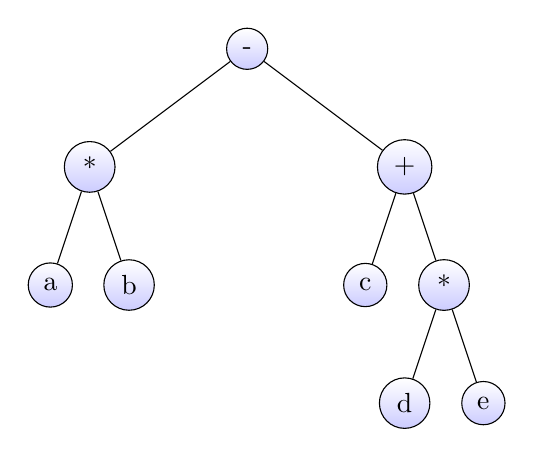
\begin{tikzpicture}[
			auto,
			level 1/.style={sibling distance=40mm},
			level 2/.style={sibling distance=10mm},
			every node/.style = {shape=circle,
				draw, align=center,
				top color=white, bottom color=blue!20}]
			\node[circle,draw] {-}
			child
			{
				node[circle,draw] {*}
				child
				{
					node[circle,draw] {a}	
				}
				child
				{
					node[circle,draw] {b}	
				}
			}
			child
			{
				node[circle,draw] {+}
				child
				{
					node[circle,draw] {c}
				}
				child
				{
					node[circle,draw] {*}
					child
					{
						node[circle,draw] {d}	
					}
					child
					{
						node[circle,draw] {e}	
					}
				}
			}
			;
			\end{tikzpicture}
		}
	\end{center}
    \end{frame}
    
    \begin{frame}
   	\frametitle{Normal/Standart Way - Suffix Notation}
	   	\begin{center}
	   	{\large
   			When we travel the tree in inorder (left-root-right), we generate the Suffix Notation.}\\\vspace{0.5cm}{\Large
   			In this case Suffix Notation is $a*b-(c+d*e)$
   		}
   		
   		{\small
   			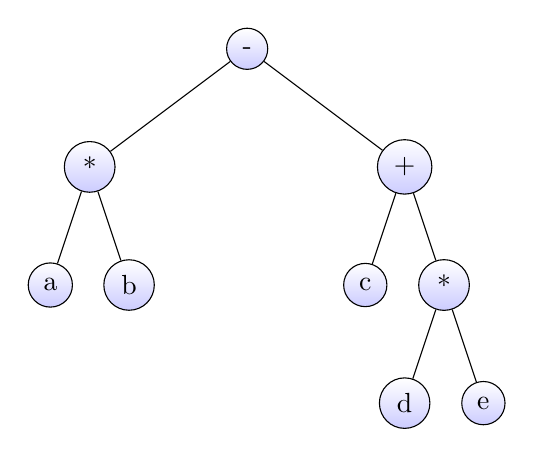
\begin{tikzpicture}[
   			auto,
   			level 1/.style={sibling distance=40mm},
   			level 2/.style={sibling distance=10mm},
   			every node/.style = {shape=circle,
   				draw, align=center,
   				top color=white, bottom color=blue!20}]
   			\node[circle,draw] {-}
   			child
   			{
   				node[circle,draw] {*}
   				child
   				{
   					node[circle,draw] {a}	
   				}
   				child
   				{
   					node[circle,draw] {b}	
   				}
   			}
   			child
   			{
   				node[circle,draw] {+}
   				child
   				{
   					node[circle,draw] {c}
   				}
   				child
   				{
   					node[circle,draw] {*}
   					child
   					{
   						node[circle,draw] {d}	
   					}
   					child
   					{
   						node[circle,draw] {e}	
   					}
   				}
   			}
   			;
   			\end{tikzpicture}
   		}
   	\end{center}
   	\end{frame}
   	\begin{frame}
   		\frametitle{Reverse Polish Notation - Postfix Notation}
   		\begin{center}
   			{\large
   				When we travel the tree in postorder (root-left-right), we generate the Postfix Notation.}\\\vspace{0.5cm}{\Large
   				In this case Postfix Notation is $- * a b + c * d e$
   			}
   		
   		{\small
   			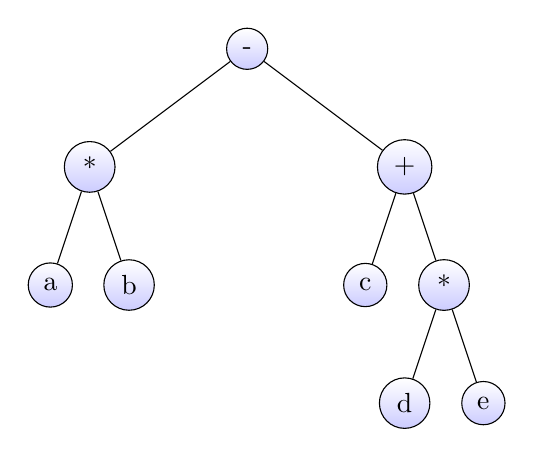
\begin{tikzpicture}[
   			auto,
   			level 1/.style={sibling distance=40mm},
   			level 2/.style={sibling distance=10mm},
   			every node/.style = {shape=circle,
   				draw, align=center,
   				top color=white, bottom color=blue!20}]
   			\node[circle,draw] {-}
   			child
   			{
   				node[circle,draw] {*}
   				child
   				{
   					node[circle,draw] {a}	
   				}
   				child
   				{
   					node[circle,draw] {b}	
   				}
   			}
   			child
   			{
   				node[circle,draw] {+}
   				child
   				{
   					node[circle,draw] {c}
   				}
   				child
   				{
   					node[circle,draw] {*}
   					child
   					{
   						node[circle,draw] {d}	
   					}
   					child
   					{
   						node[circle,draw] {e}	
   					}
   				}
   			}
   			;
   			\end{tikzpicture}
   		}
   	\end{center}
   	\end{frame}
   	\begin{frame}
   		\frametitle{Polish Notation - Prefix Notation}
   		\begin{center}
   			{\large
   				When we travel the tree in postorder (right-left-root), we generate the Prefix Notation.}\\\vspace{0.5cm}{\Large
   				In this case Prefix Notation is $d e * c + a b * -$
   			}
   		{\small
   			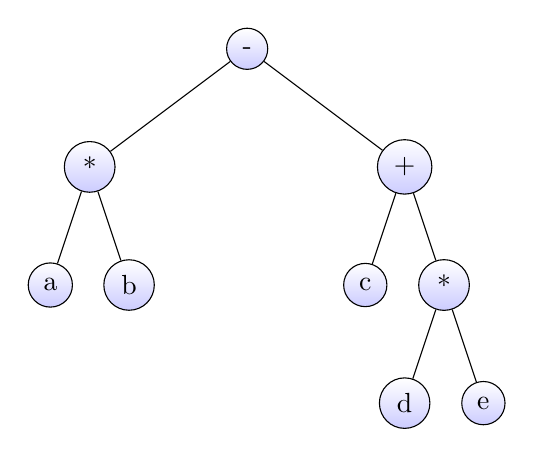
\begin{tikzpicture}[
   			auto,
   			level 1/.style={sibling distance=40mm},
   			level 2/.style={sibling distance=10mm},
   			every node/.style = {shape=circle,
   				draw, align=center,
   				top color=white, bottom color=blue!20}]
   			\node[circle,draw] {-}
   			child
   			{
   				node[circle,draw] {*}
   				child
   				{
   					node[circle,draw] {a}	
   				}
   				child
   				{
   					node[circle,draw] {b}	
   				}
   			}
   			child
   			{
   				node[circle,draw] {+}
   				child
   				{
   					node[circle,draw] {c}
   				}
   				child
   				{
   					node[circle,draw] {*}
   					child
   					{
   						node[circle,draw] {d}	
   					}
   					child
   					{
   						node[circle,draw] {e}	
   					}
   				}
   			}
   			;
   			\end{tikzpicture}
   		}
   	\end{center}
   	\end{frame}

	\begin{frame}
	\frametitle{Math/Informatics Nature}
		Each of these ways have pluses and minuses. 
	\end{frame}

	\begin{frame}
	\frametitle{Comparing}
       {\footnotesize   
       \begin{tabularx}{\textwidth}{c|c|c|c}
                         & Pre- & Post- & In-\\
          \hline
          Pre- &  & & \\
          Post- &  & & \\
          In- &  & & \\
          \hline
       \end{tabularx}
       }
	\end{frame}

	\begin{frame}
	\frametitle{Aim}
	I want to solve expression with unreal (defined by user) operators where the solving function doesn't now for any operators.\\
	For these aim I must make schema for data structuring of program and I must think for abstract algorithms.
	Let's start!
	\end{frame}
	
	\begin{frame}
	\frametitle{First step}
	    \begin{center}
        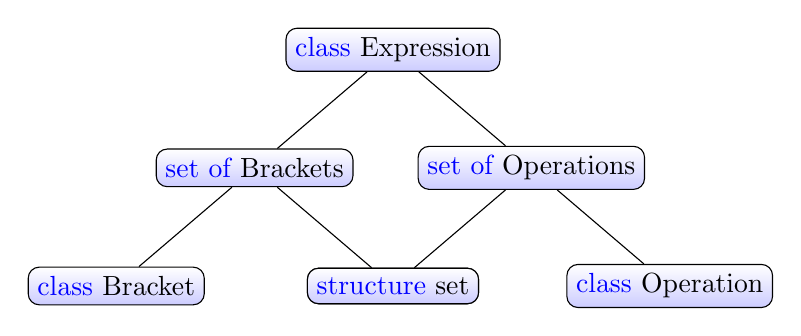
\begin{tikzpicture}[sibling distance=10em,
          every node/.style = {shape=rectangle, rounded corners,
            draw, align=center,
            top color=white, bottom color=blue!20}]]
          \node {\textcolor{blue}{class} Expression}
            child 
            { 
                node {\textcolor{blue}{set of} Brackets} 
                child
                { 
                    node {\textcolor{blue}{class} Bracket}
                }
                child
                { 
                    node {\textcolor{blue}{structure} set}
                }
            }
            child 
            { 
                node {\textcolor{blue}{set of} Operations}
                child
                { 
                    node {\textcolor{blue}{structure} set}
                }
                child
                { 
                    node {\textcolor{blue}{class} Operation}
                }
            };
        \end{tikzpicture}
        \end{center}
	\end{frame}
	
	\begin{frame}
	\frametitle{I divide the problem, can I divide more?}
	    \begin{center}
        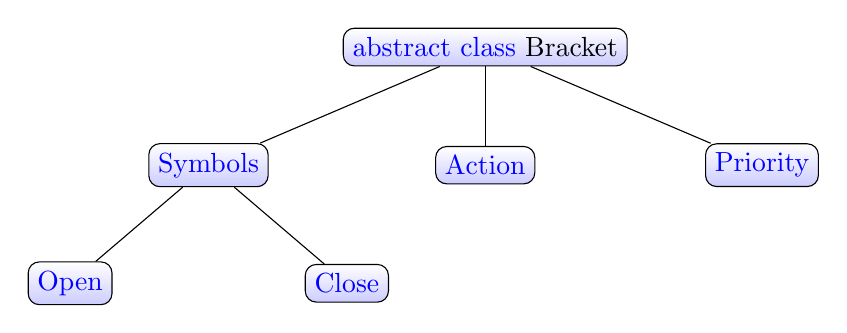
\begin{tikzpicture}[sibling distance=10em,
        every node/.style = {shape=rectangle, rounded corners,
        draw, align=center,
        top color=white, bottom color=blue!20}]]
	        \node {\textcolor{blue}{abstract class} Bracket}
                child
                {
                    node {\textcolor{blue}{Symbols}}
                    child
                    {
                        node {\textcolor{blue}{Open}}
                    }
                    child
                    {
                        node {\textcolor{blue}{Close}}
                    }
                }
                child
                {
                    node {\textcolor{blue}{Action}}
                }
                child
                {
                    node {\textcolor{blue}{Priority}}
                };
        \end{tikzpicture}
        \end{center}
	\end{frame}
	\begin{frame}
	\frametitle{And more?}
	    \begin{center}
        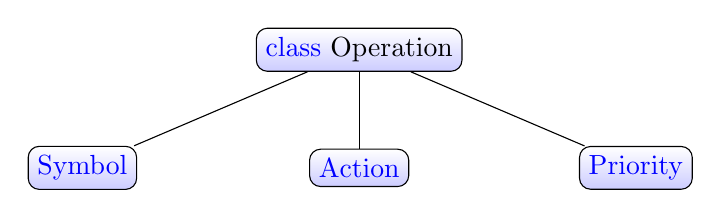
\begin{tikzpicture}[sibling distance=10em,
        every node/.style = {shape=rectangle, rounded corners,
        draw, align=center,
        top color=white, bottom color=blue!20}]]
	        \node {\textcolor{blue}{class} Operation}
                    child
                    {
                        node {\textcolor{blue}{Symbol}}
                    }
                    child
                    {
                        node {\textcolor{blue}{Action}}
                    }
                    child
                    {
                        node {\textcolor{blue}{Priority}}
                    };
        \end{tikzpicture}
        \end{center}
	\end{frame}
	\begin{frame}
	\frametitle{OK, this divide is enough! But how can I continue?}
	    \begin{center}
	    {\LARGE
	        Now we must think on \textcolor{blue}{algorithms}! \\
	        How to calculate the expression?
	    }
	    \end{center}
	\end{frame}
	\begin{frame}
		\frametitle{What is the tree of expression?}
		\begin{block}{example}
			a*b-(c+d*e)
		\end{block}
		\begin{block}{tree of expression}
			
			\begin{center}
			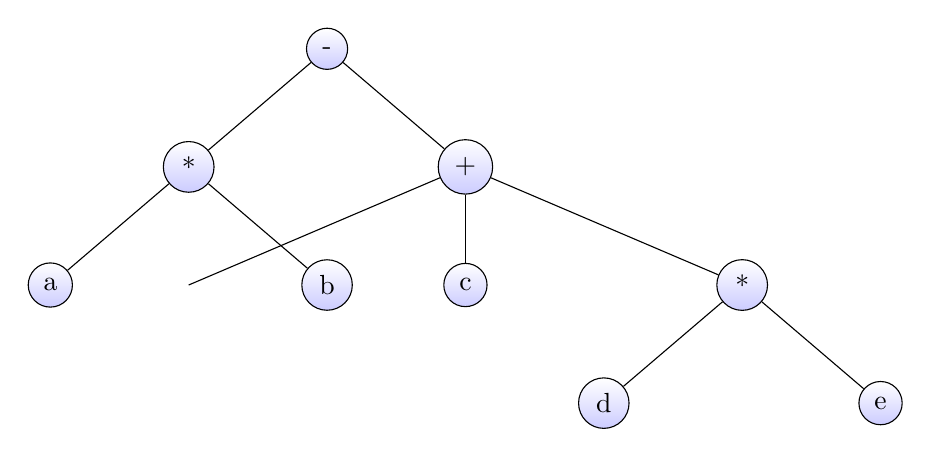
\begin{tikzpicture}[sibling distance=10em,
			every node/.style = {shape=circle,
				draw, align=center,
				top color=white, bottom color=blue!20}]]
			\node {-}
			child
			{
				node {*}
				child
				{
					node {a}	
				}
				child
				{
					node {b}	
				}
			}
			child
			{
				node {+}
				child {}
				child
				{
					node {c}
				}
				child
				{
					node {*}
					child
					{
						node {d}	
					}
					child
					{
						node {e}	
					}
				}
			}
			;
			\end{tikzpicture}
			\end{center}
		\end{block}
	\end{frame}
	\begin{frame}
    \frametitle{Analyze to find the best}
	    \begin{center}
	    	We analyzed expressions and we understand \\
	    	{\LARGE the standard way to represent expression is not effectively!} \\
	    	What next?
	    \end{center}
	    First 2 ways to solve the expression which we found are:\\
	    \begin{itemize}
	        \item Reverse Polish Notation
	        \item By Recursively
	    \end{itemize}
	\end{frame}
	
	\begin{frame}
		\frametitle{Reverse Polish Notation}
		\begin{center}
			\begin{block}{example}
				{\Large a * b - (c + d * e) } (in Suffix notation, normal way) \\
				{\Large - * a b + c * d e } (in Prefix notation, Reverse Polish notation)				
			\end{block}
		\end{center}
	\end{frame}
	
	\begin{frame}
	\frametitle{Resources}
	\end{frame}

\end{document}
